\documentclass{article}
\usepackage[utf8]{inputenc}
\usepackage{indentfirst}
\usepackage{amsmath}
\usepackage{graphicx}
\usepackage{subcaption}
\usepackage{placeins}
\usepackage{tabularx}
\usepackage{array}
\usepackage{enumitem}
\usepackage{textcomp} 
\usepackage[colorlinks]{hyperref} 

\title{Can a Shallow Ice Approximation - Degree Day Temperature Model Be Used to Model the Water Output of Alpine Glaciers?}

\author{Kieran Stone}
\date{4/30/2025}

\begin{document}

\maketitle

\section*{Abstract}

\section{Introduction}
\subsection{Importance of Glacial Melting in Mountain Hydrology}
Glacial melting plays a significant role in the hydrology of mountain catchment areas as shown in (Fountain \& Tangborn, 1985). In order to 
understand how the hydrology of these mountain catchment areas will evolve as glaciers melt and retreat, scientists create computer models to predict 
this evolution. The runoff from these mountain catchments is often used as a water source for downstream communities (Barnett et al., 2005). As shown in 
(Fountain \& Tangborn, 1985), basins with greater glaciation produce more runoff. As the glaciers in these basins melt and retreat, 
change in meltwater patterns and amounts can affect communities that rely on it in a variety of ways.

\subsection{Role of Numerical Modeling in Understanding Glacial Runoff}
One of the best ways to understand how glaciers affect the runoff of the basins that they occupy is by using computer models. 
Scientists have been using computers to model glaciers for several decades, 
such as (Iken, 1981). As computational resources have grown, these models have grown in complexity and resolution, leading 
to highly computationally expensive models. These models have proved to be very accurate in modeling the past and present state of a variety 
of glacier types all around the world(Eis et al., 2021; Farinotti et al., 2020).

\subsection{Challenges in Computational Modeling of Glaciers}
Many of these more advanced models can be quite complex to run because they require a variety of input parameters and different configurations to run the model. The 
goal of this paper is to write a simple Shallow Ice Approximation (SIA)-Mass Balance model that is easy to run and understand while still 
being generalizable to a variety of small mountain glaciers. The advantage of using much more advanced models is that they often do 
a much better job at modeling the ice dynamics of glaciers. For some glaciers such as marine calving glaciers, accurate ice dynamics are 
crucial for accurate modeling, as shown in (Amaral et al., 2020). However, on smaller mountain glaciers, modeling in three dimensions is often 
unnecessary and simpler models such as the SIA can be used (Le Meur et al., 2004). This paper will compare the results of a simple SIA-Mass Balance model to the 
results of the Open Global Glacier Model (OGGM)(Maussion et al., 2019), a more advanced model using the ice-thickness continuity equation to model ice dynamics.

\section{Literature Review}
\subsection{Prior Research on SIA vs. Stokes Models}
Table 1 shows that there are significant differences in computational time between an SIA model and a Stokes model. 
(Le Meur et al., 2004) show that there are some instances where SIA models do significantly worse than 
Stokes models, such as glaciers on steep slopes and in narrow valleys, because the SIA equations only approximate the Stokes 
equations. One of these approximations is to ignore horizontal stress gradients which can cause an SIA model to deviate from a Stokes model 
significantly in predicted glacier flow and expansion. In the 2D model, the bed characteristics and slope become the limiting factor of the SIA model.
They found instances in which the SIA model performed well 
compared to Stokes model--particularly for large flat glaciers with relatively free edges. One thing to note about (Le Meur et al., 2004) is 
that the authors are looking at the shape, area, and velocity profile of the glacier, whereas this study will focus on the water runoff 
(surface mass loss) of the glacier.
\begin{table}[ht]
    \centering
    \begin{tabular}{lcc}
      \hline
      \textbf{Metric} & \textbf{SIA model} & \textbf{Full Stokes model} \\
      \hline
      CPU time (2D free surface)                & $<1$ min        & 2 hrs    \\
      CPU time (3D free surface)                & 2 min  & 4 days    \\
      Upper free surface        & 1.15-1.2×    &    \\
      Relevant surface velocities    & 2.0×   &      \\
      Max velocity (3D model)               & 1.9×         &       \\
      Max velocity (2D model)               & 1.3×         &        \\
      Cross-sectional area        & 1.5×         &       \\
      \hline
    \end{tabular}
    \caption{Summary of key performance and output metric differences between the SIA and Stokes models (Le Meur et al., 2004). (×) indicates ratio of the metric between the SIA and Stokes models.}
    \label{tab:sia_vs_stokes}
  \end{table}
\FloatBarrier  
  
\subsection{Applying SIA Models to Alpine Glaciers}
    There are several papers, (Le Meur \& Vincent, 2003; Le Meur et al., 2004; Kessler et al., 2006), that use an SIA model for alpine glaciers. The consensus 
from those papers is that SIA models only work well on alpine glaciers with a low aspect ratio, defined as the thickness-to-extent ratio 
(Le Meur et al., 2004). The glacier used by this study will have a low aspect ratio and therefore the SIA equations should work well to model it.
\subsection{Applying SIA Models to Glacial Runoff}
    Additionally, there is precedent for using an SIA-Mass Balance model for modeling water runoff from glaciers (Naz et al., 2014). This paper used 
an SIA model to approximate the ice dynamics and a mass balance model to approximate the accumulation and ablation patterns on the glacier. 
As shown in their paper, the SIA model was able to accurately predict the glacier, and the coupled hydrological model was able to predict 
the stream flow accurately---only overestimating the July flow by an average of 13\% and underestimating the August and September flow by an 
average of 2\%.

\section{Thesis Question}
\paragraph{}
\noindent\textit{\textbf{Can a simple SIA - Mass Balance model be used to model the water runoff of small mountain glaciers?}}
% How much do ice dynamics affect the model result when modeling the water runoff of small mountain glaciers? 
\paragraph{}
If using a simple one dimensional SIA-Mass Balance model on small mountain glaciers (with low aspect ratios), the mass balance profile will have a 
much larger effect on the output of the model and its overall accuracy than the modeled ice dynamics. The results of the SIA-Mass Balance 
model and the OGGM model will be compared to the actual stream flow data to answer this question.
\subsection{Study Site: South Cascade Glacier, Washington State}
This study will focus on modeling the South Cascade Glacier in the North Cascades region of Washington State. This glacier is 
roughly 1.68 km$^2$ with widths ranging from 400m-1200m. It has a mean elevation of roughly 1900m, (GLIMS Consortium, 2005) faces North, has 
an average thickness of 99m, and a maximum thickness of 195m (GlaThiDa Consortium, 2020). The glacier is 
not overly steep (average slope of 7.14 degrees along this studies centerline in 2021), and has a low aspect ratio 
(thickness to extent ratio). Therefore an SIA model should be able to accurately model its ice dynamics. On the other hand, 
the glacier is large enough to exhibit some movement and produce a measurable amount of runoff throughout the year.

\begin{figure}[h!]
    \centering
    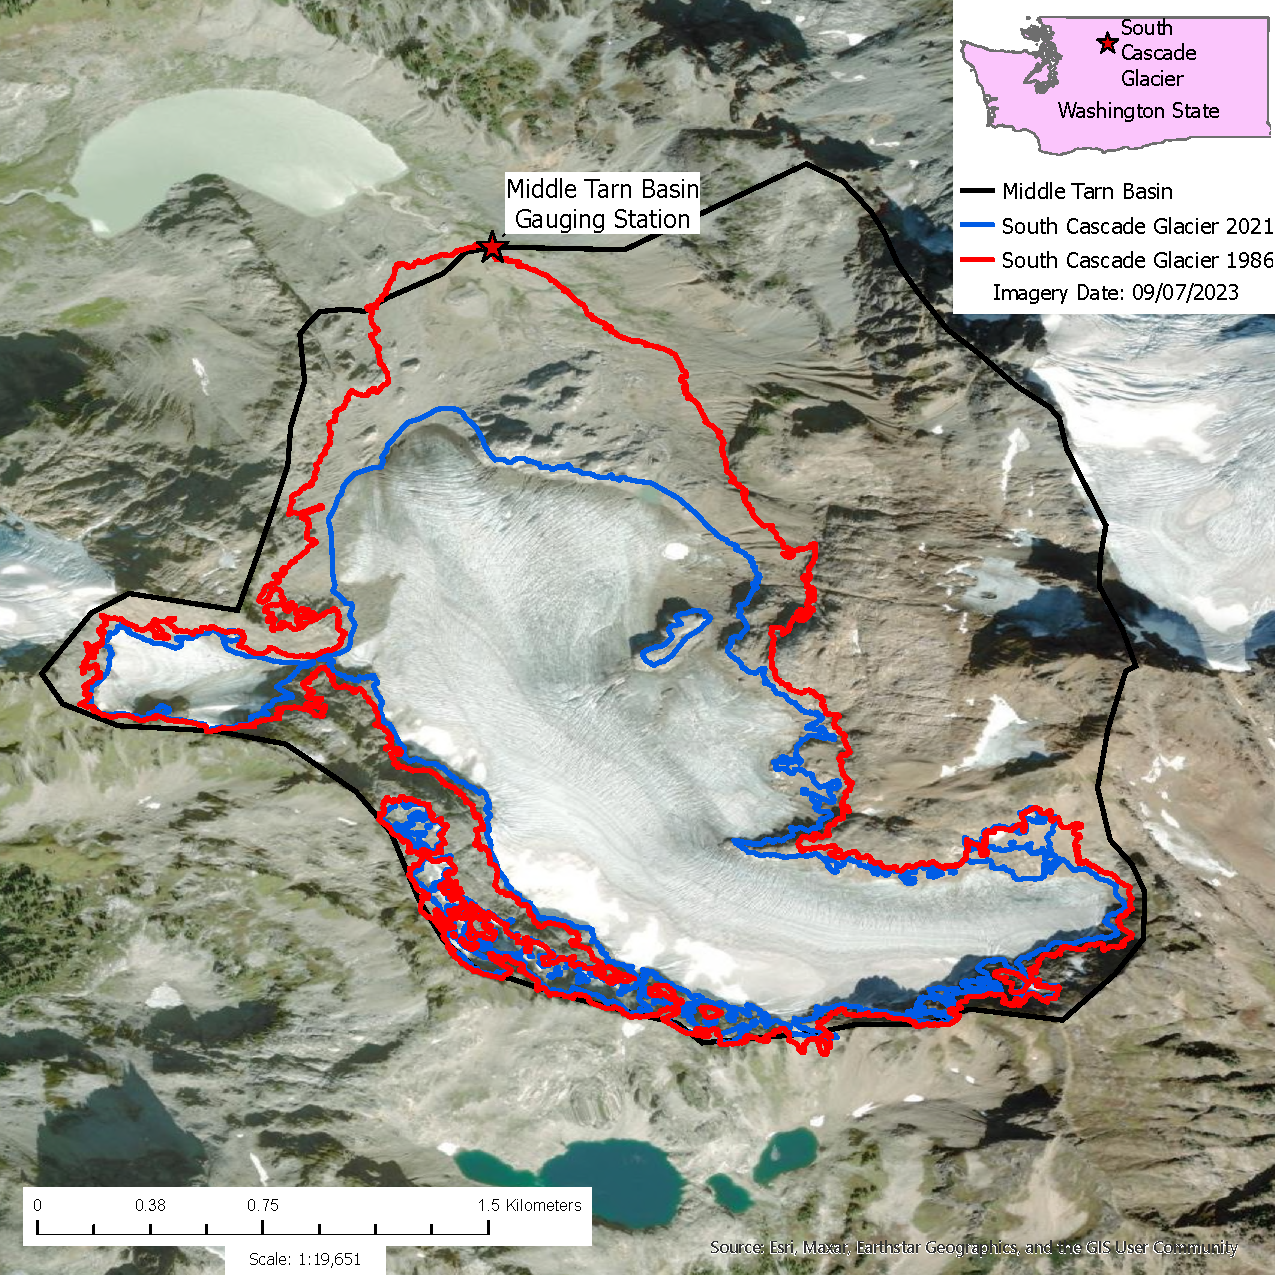
\includegraphics[width=\textwidth]{Plots/SouthCascadeGlacierMap.pdf}
    \caption{Map of the South Cascade Glacier in the North Cascades of Washington.}
    \label{fig:south_cascade_glacier}
\end{figure}
\FloatBarrier

\begin{table}[h!]
    \centering
    \begin{tabularx}{\textwidth}{|c|X|}
        \hline
        Symbol & Description \\
        \hline
        $Z_g$ & Glacier surface altitude (m) \\
        ELA & Equilibrium line altitude (m)\\
        $\gamma$ & Spinup mass balance equation gradient (m/year)\\
        $Y$ & Current year \\
        $Q$ & Ice flux ($\text{m}^2/\text{day}$)\\
        $A$ & Flow rate factor ($5.87*10^{-19}\text{Pa}^{-3}\text{day}^{-1}$) \\
        $n$ & Flow law exponent (3) \\
        $\rho$ & Density of ice ($917\text{kg/m}^3$) \\
        $g$ & Acceleration due to gravity ($9.81\text{ m/s}^2$) \\
        $\frac{\partial z_s}{\partial x}$ & Slope of glacier \\
        $H$ & Ice thickness (m)\\
        $T$ & Temperature ($^\circ$C) \\
        m.w.e & meters water equivalent \\
        $M_{s}$ & Snow melt factor ($\text{m.w.e}/^\circ\text{C}/\text{day}$) \\
        $M_{i}$ & Ice melt factor ($\text{m.w.e}/^\circ\text{C}/\text{day}$) \\
        $P$ & Precipitation (m) \\
        $\alpha$ & Precipitation conversion factor \\
        $b_s$ & Summer mass balance (m/day) \\
        $b_w$ & Winter mass balance (m/day) \\
        ${Accum}_{l}$ & Accumulation factor lower bound ($\text{m.w.e}_{\text{ice}}/\text{m.w.e}_{\text{precipitation}}$) \\
        ${Accum}_{u}$ & Accumulation factor upper bound ($\text{m.w.e}_{\text{ice}}/\text{m.w.e}_{\text{precipitation}}$) \\
        $S_{d}$ & Snow depth (m.w.e) \\
        $S_{mv}$ & Snow melt volume ($\text{m.w.e}^3$) \\
        ${Area}_{b}$ & Basin area ($\text{m}^2$) \\
        ${Area}_{g} $ & Glacier area ($\text{m}^2$) \\
        $R_{v}$ & Rain volume ($\text{m}^3$) \\
        $G_{mv}$ & Glacial melt volume ($\text{m.w.e}^3$) \\
        \hline
    \end{tabularx}
    \caption{Symbols Table}
    \label{tab:symbols_table}
\end{table}
\FloatBarrier

\section{Methods}
\subsection{Model Development}
\subsubsection{Model Overview}
\textbf{Model Structure:}
\begin{enumerate}[leftmargin=2cm]
    \item SIA ice dynamics model
    \item Temperature degree day and precipitation mass balance model
    \item Temperature degree day and precipitation (snow fall/melt and rain) model
\end{enumerate}

There are two sections to the complete model run, the spinup run and the data driven run. The spinup section of the model runs for 500 years and aims to replicate the 
state of the glacier in 1984 when weather data becomes readily available. The spinup run starts with the bed topography and no ice and uses a simple mass balance 
equation to accumulate ice to simulate the glacier state in 1984. The data driven run starts in 1984 with the simulated spinup glacier and applies a temperature and 
precipitation driven mass balance model to model how the glacier changes until 2024 when the weather data ends. The data driven run also contains the precipitation model to calculate the runoff 
from snow melt and rainfall.

\subsubsection{Spinup Run}
This section uses a simple mass balance equation 1 to model the accumulation and ablation of the glacier.
\begin{equation}((Z_g-\text{ELA})*\gamma)/365.25\label{tab:simple_mb_eq}\end{equation}
A $\gamma$ of 0.0309 is used to calculate the mass balance change in meters per day. When the spinup hits the year 1900 the ELA is shifted up from 1903m to 1930m to force the 
glacier to retreat. 

\subsubsection{Data Driven Run Setup}
The data driven run of the model relies on a variety of data in order to run. It requires daily temperature and precipitation data, 
a bed topography, yearly glacier area, and total basin area. In order to tune the input parameters the model also needs winter and summer mass balance 
data. The model requires seven input parameters to run: ice melt factor, snow melt factor, temperature lapse rate, lower accumulation factor, upper 
accumulation factor, avalanche percentage and precipitation conversion factor. The details of how these input parameters are calibrated and used 
in the model are explained in the following sections.

\subsubsection{Ice Dynamics}
\paragraph{SIA Model}
The SIA model is a one-dimensional model that uses the shallow ice approximation equations to calculate the ice dynamics of the glacier. This model 
calculates the one dimensional ice flux of the glacier using equation 2. 
\begin{equation}Q=\frac{2A}{n+2}(\rho g|\frac{\partial z_s}{\partial x}|)^n\frac{H^5}{5}\label{tab:ice_dyn_eq}\end{equation}

\paragraph{Assumptions}
The SIA ice flux equation makes several assumptions. First, the equation is 1-dimensional, so it neglects longitudinal stress, and ice only 
flows downhill. Second, the equation assumes that there is no basal sliding of the glacier. Third, it only uses gravity as the 
driver of ice flow; it ignores other forces such as lateral and basal stress. Fourth, this equation assumes that the horizontal 
dimensions of the modeled glacier are much larger than the vertical dimensions.

\subsubsection{Mass Balance Model}
The mass balance of the glacier is calculated using temperature and precipitation data from the Diablo Dam weather station at 272m. The 
temperature at the glacier is calculated by using a month-specific lapse rate. 
The precipitation at the glacier is calculated by adjusting the precipitation at Diablo Dam with a precipitation conversion factor of 1.58 
(Rasmussen, 2009). The ablation of the glacier is modeled using a combination of an ice melt factor and a snow melt factor. Above the ELA
the ablation is calculated by equation 3 for $T>0$. The ELA is computed by finding the elevation at which the previous year's mass balance 
changes from positive to negative.
\begin{equation}b_s=T*M_{s}\label{tab:summer_mb_below_ela_eq}\end{equation}
Below the ELA the ablation is calculated by equation 4 for $T>0$.
\begin{equation}b_s=T*(M_{s}+((ELA-Z_g)/(ELA-min(Z_g)))*(M_{i}-M_{s}))\label{tab:summer_mb_above_ela_eq}\end{equation}
The result of this equation is the snow melt factor being used at the ELA and a linear increase in the melt factor until it hits the ice melt 
factor at the base of the glacier. This set of equations assumes that in the accumulation zone (above the ELA) the glacier surface is always snow year 
round, and below the ELA the glacier surface transitions from snow to ice as you decrease in elevation.
\paragraph{}
The accumulation of the glacier is calculated using equation 5 for $T<0$.
\begin{equation}b_w=P*\alpha*({Accum}_{l}+((Y-1984)/(2024-1984))*({Accum}_{l}-{Accum}_{u}))\label{tab:winter_mb_eq}\end{equation}
This equation starts the accumulation factor at the accumulation factor lower bound at the start of the data driven run in 1984 and linearly 
increases it to accumulation factor upper bound by the end of the run in 2024.

\subsubsection{Precipitation Model}
\paragraph{Snow Model}
The snow model uses precipitation and temperature data to accumulate and melt snow. To calculate the change in snow depth equation 6 is used.
\begin{equation}S_{d} += 
\begin{cases} 
  P*\alpha & T \leq 0,\\
  -\text{min}(|M_{s}*T|,S_{d}) &  T > 0
\end{cases}\label{tab:snow_depth_eq}\end{equation}
The snow melt calculation is constrained so that there cannot a negative snow depth. 
The total volume of snow melt is calculated by equation 7.
\begin{equation}S_{mv}=(M_{s}*T)*({Area}_{b}-{Area}_{g})\label{tab:snow_melt_eq}\end{equation}
This give us the total volume of snow melt on the non-glacierized areas of the basin. Any snow that falls on the glacier is factored into 
the glacier mass balance equations and accumulated on the glacier.
\paragraph{Rain Model}
The rain is simply modeled by $P*\alpha$ for positive temperature days. The volume of rain is calculated by equation 8.
\begin{equation}R_{v}=P*\alpha*{Area}_{b}\label{tab:rain_vol_eq}\end{equation}
This calculates the volume of rain for the whole basin because rain is not factored into the glacier mass balance model. This assumes that  that any rain 
that falls runs out of the basin on the day it falls.

% \textbf{ask mom to review this section in particular, make sure it makes sense}
\paragraph{Avalanche Model}
In order to stop snow accumulating to unrealistic depths at high elevations an avalanche model is used. This model avalanches the 
snow above 2123m once per year on a randomly chosen date between January and March, which changes every year. The amount of snow that 
avalanches is determined by the avalanche percentage parameter. On the chosen day the snow depth above 2123m is decreased by the avalanche 
percentage and that snow is evenly distributed below 1900m. The result of this is the average monthly snow depth hitting approximately 2m.w.e at its lowest point 
in September and October before starting to accumulate again. With an avalanche percentage of 0 it is approximately 5.5m.w.e 
in September and October. This decrease in snow depth yields a more realistic model and improves runoff model accuracy by about 
one percentage point. This is due to there being more snow available for melt during the summer at the lower elevations where the 
temperature is higher.

\subsubsection{Glacial Melt Model}
The glacial melt model uses the mass balance of the glacier to calculate how much volume the glacier is losing. The volume of runoff from the 
glacier is calculated by equation 9.
\begin{equation}G_{mv}=b_s*{Area}_{g}\label{tab:glacier_melt_eq}\end{equation}
\subsection{Model Calibration}
\subsubsection{Data Used for Model}
The temperature and precipitation data used for the model is from the Diablo Dam weather station at 272m (U.S. Geological Survey Benchmark Glacier Program, 2020). This data is available from 1984-2024 
and is missing 298 days of temperature data and 292 days of precipitation data. The missing temperature data was interpolated 
using the interp function from the numpy python library (Harris et al., 2020), the missing precipitation data was assumed to be 0. Since the Diablo Dam
weather station is at a significantly lower altitude than the South Cascade Glacier a lapse rate is applied to the temperature data. This lapse 
rate was empirically calculated using data (Baker et al., 2018) from a weather station at 1830m next to the South Cascade Glacier. This data is available daily from 
2010-2018. Using these two sets of data an monthly average lapse rate was calculated between Diablo Dam and the South Cascade Glacier (Table 3). 
\begin{table}[h!]
    \centering
    \small
    \begin{tabular}{|*{6}{c|}}
      \hline
      Jan & Feb & Mar & Apr & May & Jun \\ 
      \hline
      $-3.35$ & $-5.45$ & $-5.77$ & $-6.79$ & $-6.61$ & $-6.28$ \\
      \hline
    \end{tabular}
    \begin{tabular}{|*{6}{c|}}
      \hline
      Jul & Aug & Sep & Oct & Nov & Dec \\ 
      \hline
      $-5.30$ & $-5.35$ & $-4.95$ & $-4.94$ & $-4.73$ & $-4.52$ \\
      \hline
    \end{tabular}
    \caption{Monthly lapse rates ($^\circ$C/km)}
    \label{tab:temp_lapse_rates}
  \end{table}
\FloatBarrier
% \paragraph{}
The glacier area data used in the model is from the USGS (U.S. Geological Survey Benchmark Glacier Program, 2020). The basin area was calculated from the basin outline shown in Figure 1.
\paragraph{}
The centerline bed topography was calculated using latitude, longitude and elevation bed topography data from Robert Jacobel (Fountain \& Jacobel, 1997). 
The ArcGIS Kriging Interpolation function (Environmental Systems Research Institute, 2011) was used to interpolate this point elevation data into a complete 
bed topography across the whole glacier. Then a line was traced down the center of the glacier using the interpolated bed and elevations 
were extracted to create the bed topography of the centerline. Finally, these latitude, longitude, and elevation points were used to create 
the one-dimensional bed topography in the model.

\subsubsection{Calibration} 
\paragraph{Spinup Calibration}
The spinup initial ELA, ELA in 1900 and $\gamma$ were optimized using the minimize function with the Nelder-Mead method from the scipy python library (Virtanen et al., 2020).
The optimization was done by minimizing the Root Mean Squared Error (RMSE) of the modeled and measured glacier ice thicknesses in 1958 and 1986. 
The measured glacier ice thickness was calculated using DEM's of the glacier in 1958 and 1986 (McNeil et al., 2019).  
The result is an average RMSE of 20.24m with RMSE's of 21.36m and 19.11m in 1958 and 1986 respectively.

\begin{equation}
    \mathrm{RMSE} = \left(\frac{\sqrt{\frac{1}{n} \sum_{i=1}^{n} \bigl(O^{1958}_i - S^{1958}_i\bigr)^2}+\sqrt{\frac{1}{n} \sum_{i=1}^{n} \bigl(O^{1986}_i - S^{1986}_i\bigr)^2}}{2} \right)*100 \label{tab:rmse_spinup_eq}
\end{equation}

\noindent where:
$$O = \text{Measured ice thicknesses}, \quad S=\text{Modeled ice thicknesses}$$

\paragraph{Summer Mass Balance Calibration}
The two input parameters that control the summer mass balance are the ice melt factor and the snow melt factor. They were calibrated using yearly summer 
mass balance data available from the USGS from 1984-2024 (U.S. Geological Survey Benchmark Glacier Program, 2020). The same minimize function used for the spinup calibration was used to 
to minimize the RMSE between the modeled mass balance and the USGS measured mass balance. The result is a RMSE of 0.52m

\begin{equation}
    \mathrm{RMSE} \;=\; \sqrt{\frac{1}{n} \sum_{i=1}^{n} \bigl(O_i - S_i\bigr)^2} \label{tab:rmse_mb_eq}
\end{equation}
    
\noindent where:
$$O = \text{Measured summer mass balance (m)}, \quad S=\text{Modeled summer mass balance (m)}$$

\paragraph{Winter Mass Balance Calibration}
There are also two factors that control the winter mass balance, the upper and lower bound accumulation factors. These were tuned using the same 
method as the summer mass balance factors using the USGS yearly winter mass balance data available from 1984-2024 (U.S. Geological Survey Benchmark Glacier Program, 2020). 
The result is an RMSE of 0.55m (\ref{tab:rmse_mb_eq}).

\paragraph{Avalance Percentage Calibration}
The avalanche percentage was optimized using the same minimize function as the mass balance parameters. Instead of minimizing the RMSE, the mean of the 
snow depth over the whole data driven model run (1984-2024) was minimized. The mean snow depth was minimized because almost all of the snow on the 
non-glacierized areas of the basin should melt during the summer. By minimizing the mean snow depth over the whole run, only the snow depth during 
the summer will be minimized since the avalanche percent cannot change the amount of snow present in the whole basin, just the elevation it is at. If 
there is more snow at lower elevations then more snow will melt during the summer.

\subsubsection{Model Comparison}
\paragraph{Running OGGM for the South Cascade Glacier}
OGGM was run using the run\_with\_hydro task from the oggm library. This model run used the GSWP3\_W5E5 historical temperature and 
precipitation data (Lange et al., 2021) to model the hydrology of the glacier from 1984-2019. The total runoff from the glacier was calculated 
using the melt\_on\_glacier\_monthly, and liq\_precip\_on\_glacier\_monthly variables. In order 
to calculate the runoff from the non-glacierized areas, \linebreak melt\_off\_glacier\_monthly, and liq\_precip\_off\_glacier\_monthly variables were averaged over the 
SIA model glacier basin area. 

\section{Results}
\subsection{Accuracy of SIA Model}
The calculated runoff of the SIA-Mass Balance model was validated using measured streamflow data from 1992-2007, consisting of 2418 
data points, which were aggregated into 91 months (Krimmel, 1993, 1994, 1995, 1996, 1997, 1998, 1999, 2000, 2001, 2002; Bidlake et al., 2004, 2005, 2007, 2010). This data was measured using 
a stream gauge located just below the glacier (refer to \hyperref[fig:south_cascade_glacier]{Figure~\ref*{fig:south_cascade_glacier}}  for location). The data is in units of mm per day averaged over the basin area (4.46$\text{km}^2$). This was  
converted to cubic meters per day and then 
summed over the month to calculate a monthly runoff. Not every month was complete, so in order to validate the model, the model runoff was saved 
for the same days as the measured data and then a daily average was calculated for each month. 
This paper will look at the model error in terms of daily average runoff per month due to the several incomplete months of data. 
This paper will use three types of error to evaluate the model, relative Root Mean Square Error (RMSE), Nash–Sutcliffe Efficiency (NSE), and Kling–Gupta Efficiency 
(KGE), defined by the equations below. 
\begin{equation}
    \mathrm{RMSE} = \frac{\sqrt{\frac{1}{N}\sum_{i=1}^{N} \left( O_i - S_i \right)^2}}{\bar{O}}*100 \label{tab:rmse_runoff_eq}
\end{equation}

\begin{equation}
    \mathrm{NSE} = 1 - \frac{\sum_{i=1}^{N}\left( O_i - S_i \right)^2}{\sum_{i=1}^{N}\left( O_i - \bar{O} \right)^2} \label{tab:nse}
\end{equation}

\begin{equation}
    \mathrm{KGE} = 1 - \sqrt{ (r-1)^2 + (\alpha-1)^2 + (\beta-1)^2 } \label{tab:kge}
\end{equation}

\noindent where:
$$O = \text{Observed data}, \quad S=\text{Simulated Data}$$
$$r = \mbox{Correlation coefficient}, \quad \alpha = \frac{\sigma_S}{\sigma_O}, \quad \beta = \frac{\mu_S}{\mu_O}$$
The results for these three methods are 29.26\%, 0.81 and 0.88 respectively. It is important to note that this error is primarily the model error for 
May-November due to the lack of runoff data outside of those months. There is one instance of January, February, March and April, and six 
instances of December. The model does much better on longer timescales where the relative RMSE of the daily average runoff 
per year drops to 15.21\%.
\begin{figure}[h!]
    \centering
    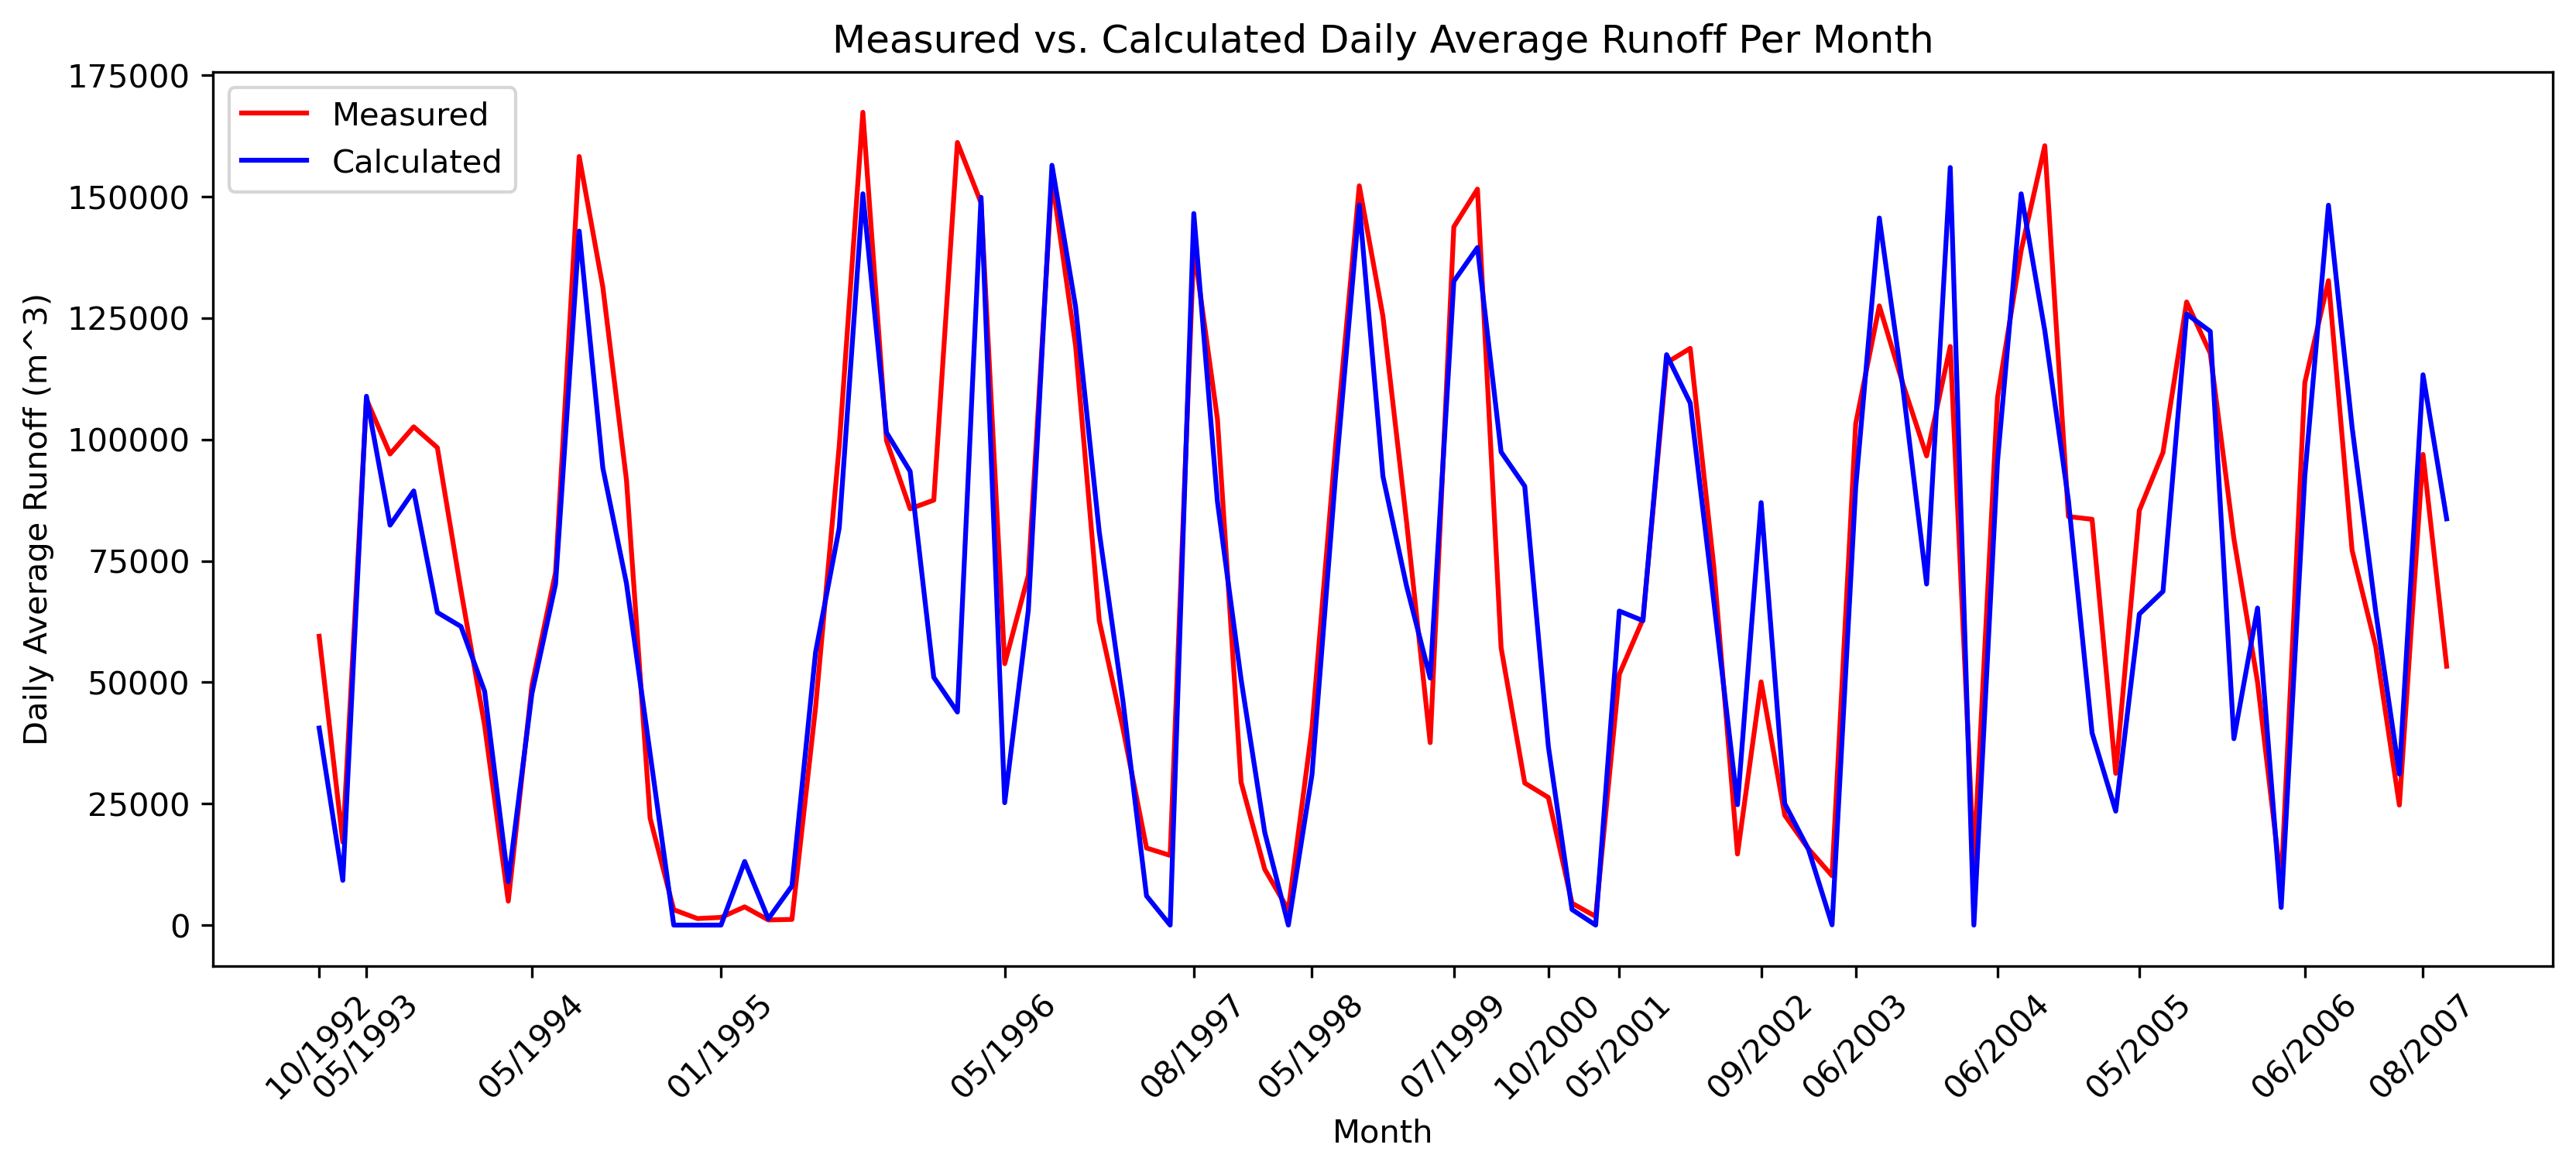
\includegraphics[width=\textwidth]{Plots/calc_vs_measured.png}
    \caption{Measured vs. Calculated runoff data from 1992-2007}
    \label{fig:calc_vs_measured}
\end{figure}
\FloatBarrier
\subsection{Accuracy of OGGM}
The RMSE(\ref{tab:rmse_runoff_eq}), NSE(\ref{tab:nse}) and KGE(\ref{tab:kge}) of OGGM are 45.96\%, 0.53 and 0.72 respectively. OGGM proved to be slightly less accurate than the SIA-Mass Balance model when 
compared to the real-world measured runoff data. 
\begin{figure}[h!]
    \centering
    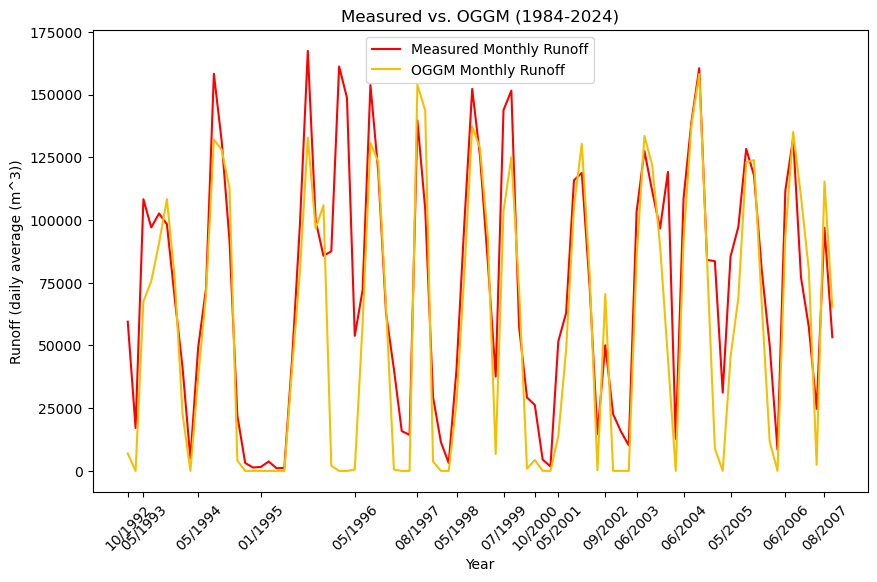
\includegraphics[width=\textwidth]{Plots/oggm_vs_measured.png}
    \caption{Measured vs. OGGM runoff data from 1992-2007}
    \label{fig:oggm_vs_measured}
\end{figure}
\FloatBarrier

\section{Discussion}
\subsection{Comparison of Model Accuracies}
The SIA-Mass Balance model is roughly 1.4 times (averaged over the three error metrics) more accurate than OGGM. One reason for the 
higher accuracy of the SIA-Mass Balance model is likely due to it 
using real-world temperature and precipitation data and OGGM using modeled climate data which is less accurate. The SIA model input 
parameters are also tuned to the local climate of the glacier which may contribute to its higher accuracy.

\begin{figure}[h!]
    \centering
    \makebox[0pt][c]{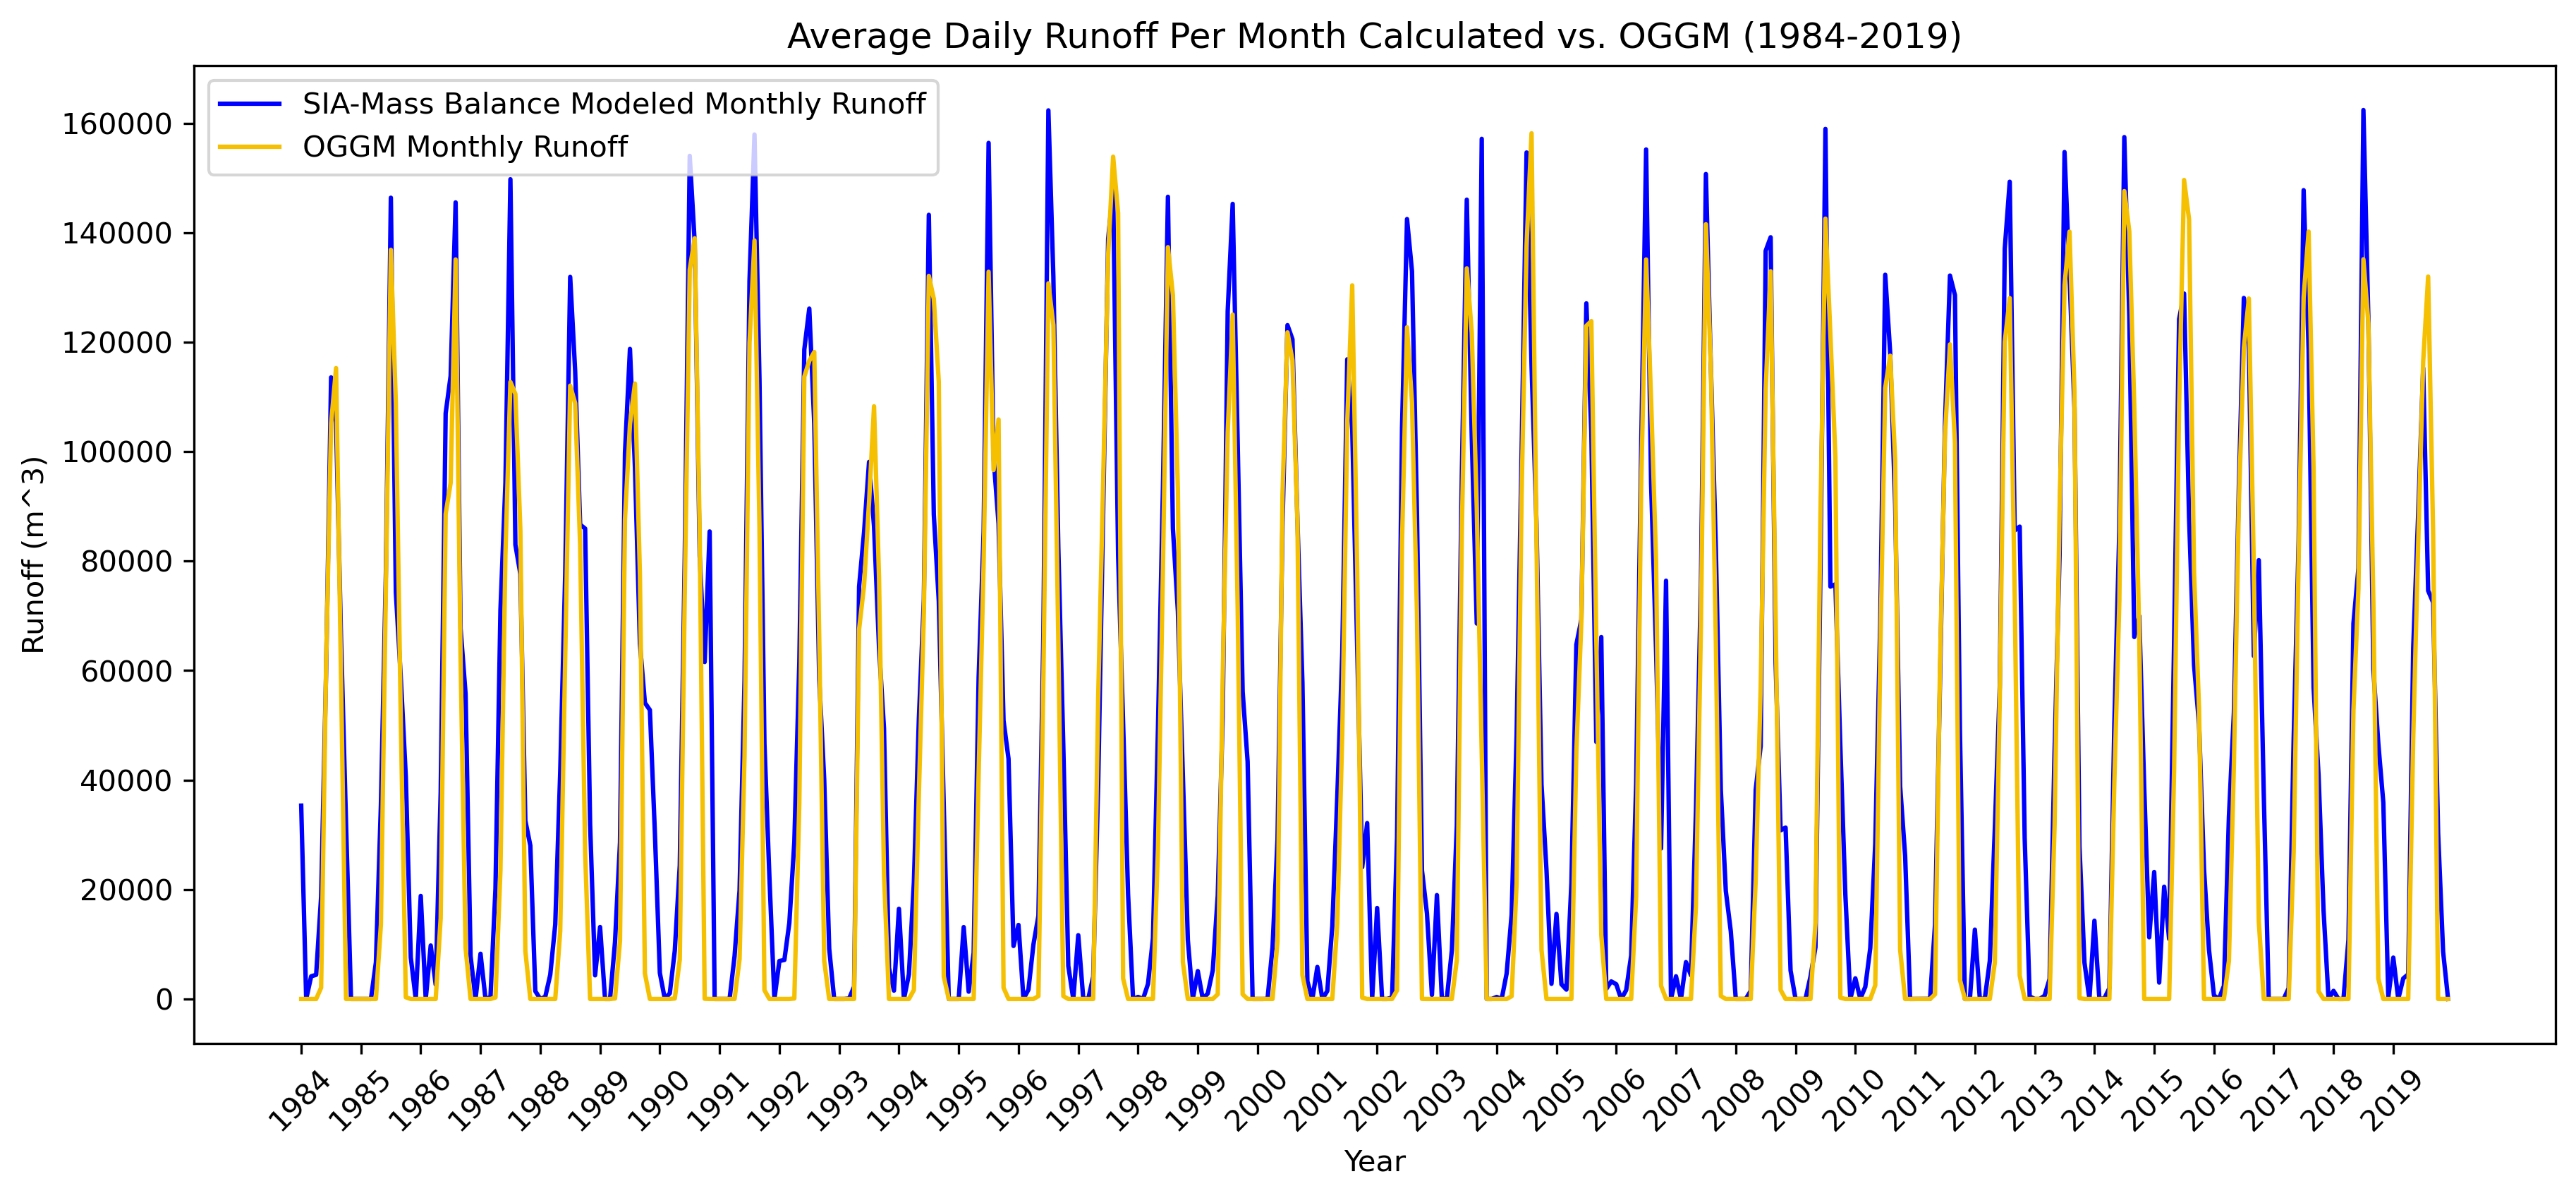
\includegraphics[width=0.8\paperwidth]{Plots/oggm_vs_calculated.png}}
    \caption{OGGM calculated daily average runoff per month compared to SIA-Mass Balance Model from 1984-2019}
    \label{fig:oggm_model_run_1984_2019}
\end{figure}
\FloatBarrier

\subsection{Spinup model error}
Looking at Figure 5 the difference in the actual glacier vs the modeled glacier at the top of the valley stands out. The modeled glacier is much thicker in this 
location compared to the actual glacier. This may be due to different accumulation patterns on the actual glacier compared to the model, or due to error in the bed 
topography data

\begin{figure}[h!]
    \centering
    \begin{subfigure}[b]{0.49\textwidth}
        \centering
        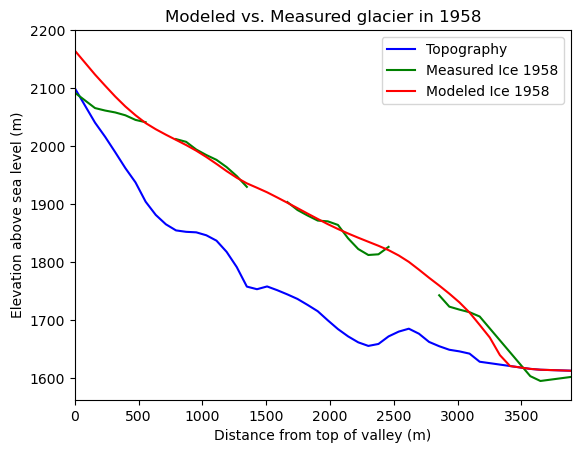
\includegraphics[width=\textwidth]{Plots/1958_glacier_comparison.png}
        \label{fig:1958_glacier_comparison}
    \end{subfigure}
    \hfill
    \begin{subfigure}[b]{0.49\textwidth}
        \centering
        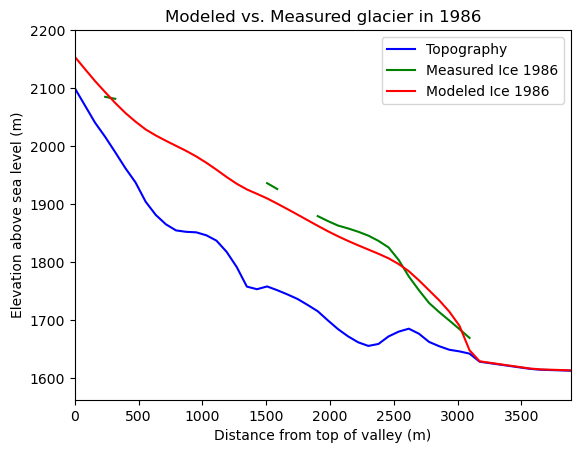
\includegraphics[width=\textwidth]{Plots/1986_glacier_comparison.png}
        \label{fig:v}
    \end{subfigure}
    \caption{Glacier from DEM compared with modeled glacier in 1958 and 1986}
    \label{fig:1986_glacier_comparison}
\end{figure}
\FloatBarrier

\subsection{Mass Balance Model Error}
% The relative RMSE of the winter and summer mass balance are 19.01\% and 13.33\% respectively.
From the missing temperature and precipitation one can note a few interesting things about the mass balance model error. There are five years 
with significant gaps (at least one month of missing data) in the temperature and precipitation data. These years are 1984 (missing December), 
1985 (missing January), 1987 (missing July), 1997 (missing March and September) and 2009 (missing May-July). The year with the highest error in 
winter mass balance is 1997 probably due to it missing March data. The measured winter mass balance that year is 3.44m, and the model calculated a 
winter mass balance of 2.65m. One possibility for this is that there was a large amount of snowfall during March of that year, but since the 
precipitation data is missing for that month, the glacier accumulation is 0. According to PRISM (PRISM Group, 2014) the South Cascade Glacier received 0.57m 
of precipitation during March 1997. Using the mass balance equations above, the accumulation on the glacier during March 1997 with 0.57m of 
precipitation would be 1m. This would increase the winter mass balance for that year from 2.65m to 3.65m. With the updated value in the modeled winter 
mass balance, the RMSE (\ref{tab:rmse_mb_eq}) drops from 0.55m to 0.54m. This 
illustrates just how important consistent and reliable weather data is for models like these because a month of missing weather data can skew the 
result.
\paragraph{}
Looking at the summer mass balance in Figure 6, the model does a good job of capturing the trends of the measured summer mass balance, but not 
the amplitude. The modeled summer mass balance consistently doesn't reach the same magnitude as the measured summer mass balance. One reason for this 
could be due to the model not taking cloud cover into effect. For years where the measured summer mass balance was particularly low, there could 
have been a lot of cloud cover which would have reduced the amount of solar radiation reaching the glacier and thus reduced the amount of melt. 
There are a lot of nuances in the weather that can change the amount of melt that occurs on the glacier. This model was designed to capture all of 
these nuances with two melt factors. This provides a good generalization of the glacier melt shown by the low RMSE for the summer mass balance data, 
but perhaps does not accurately represent the glacial melt on shorter timescales.
\begin{figure}[h!]
    \centering
    \begin{subfigure}[b]{0.49\textwidth}
        \centering
        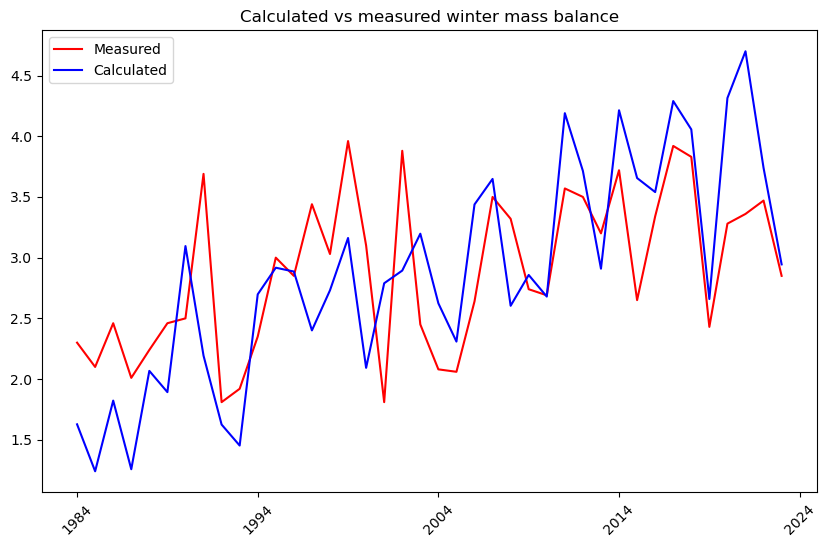
\includegraphics[width=\textwidth]{Plots/winter_mb_compare.png}
        \label{fig:winter_mb_compare}
    \end{subfigure}
    \hfill
    \begin{subfigure}[b]{0.49\textwidth}
        \centering
        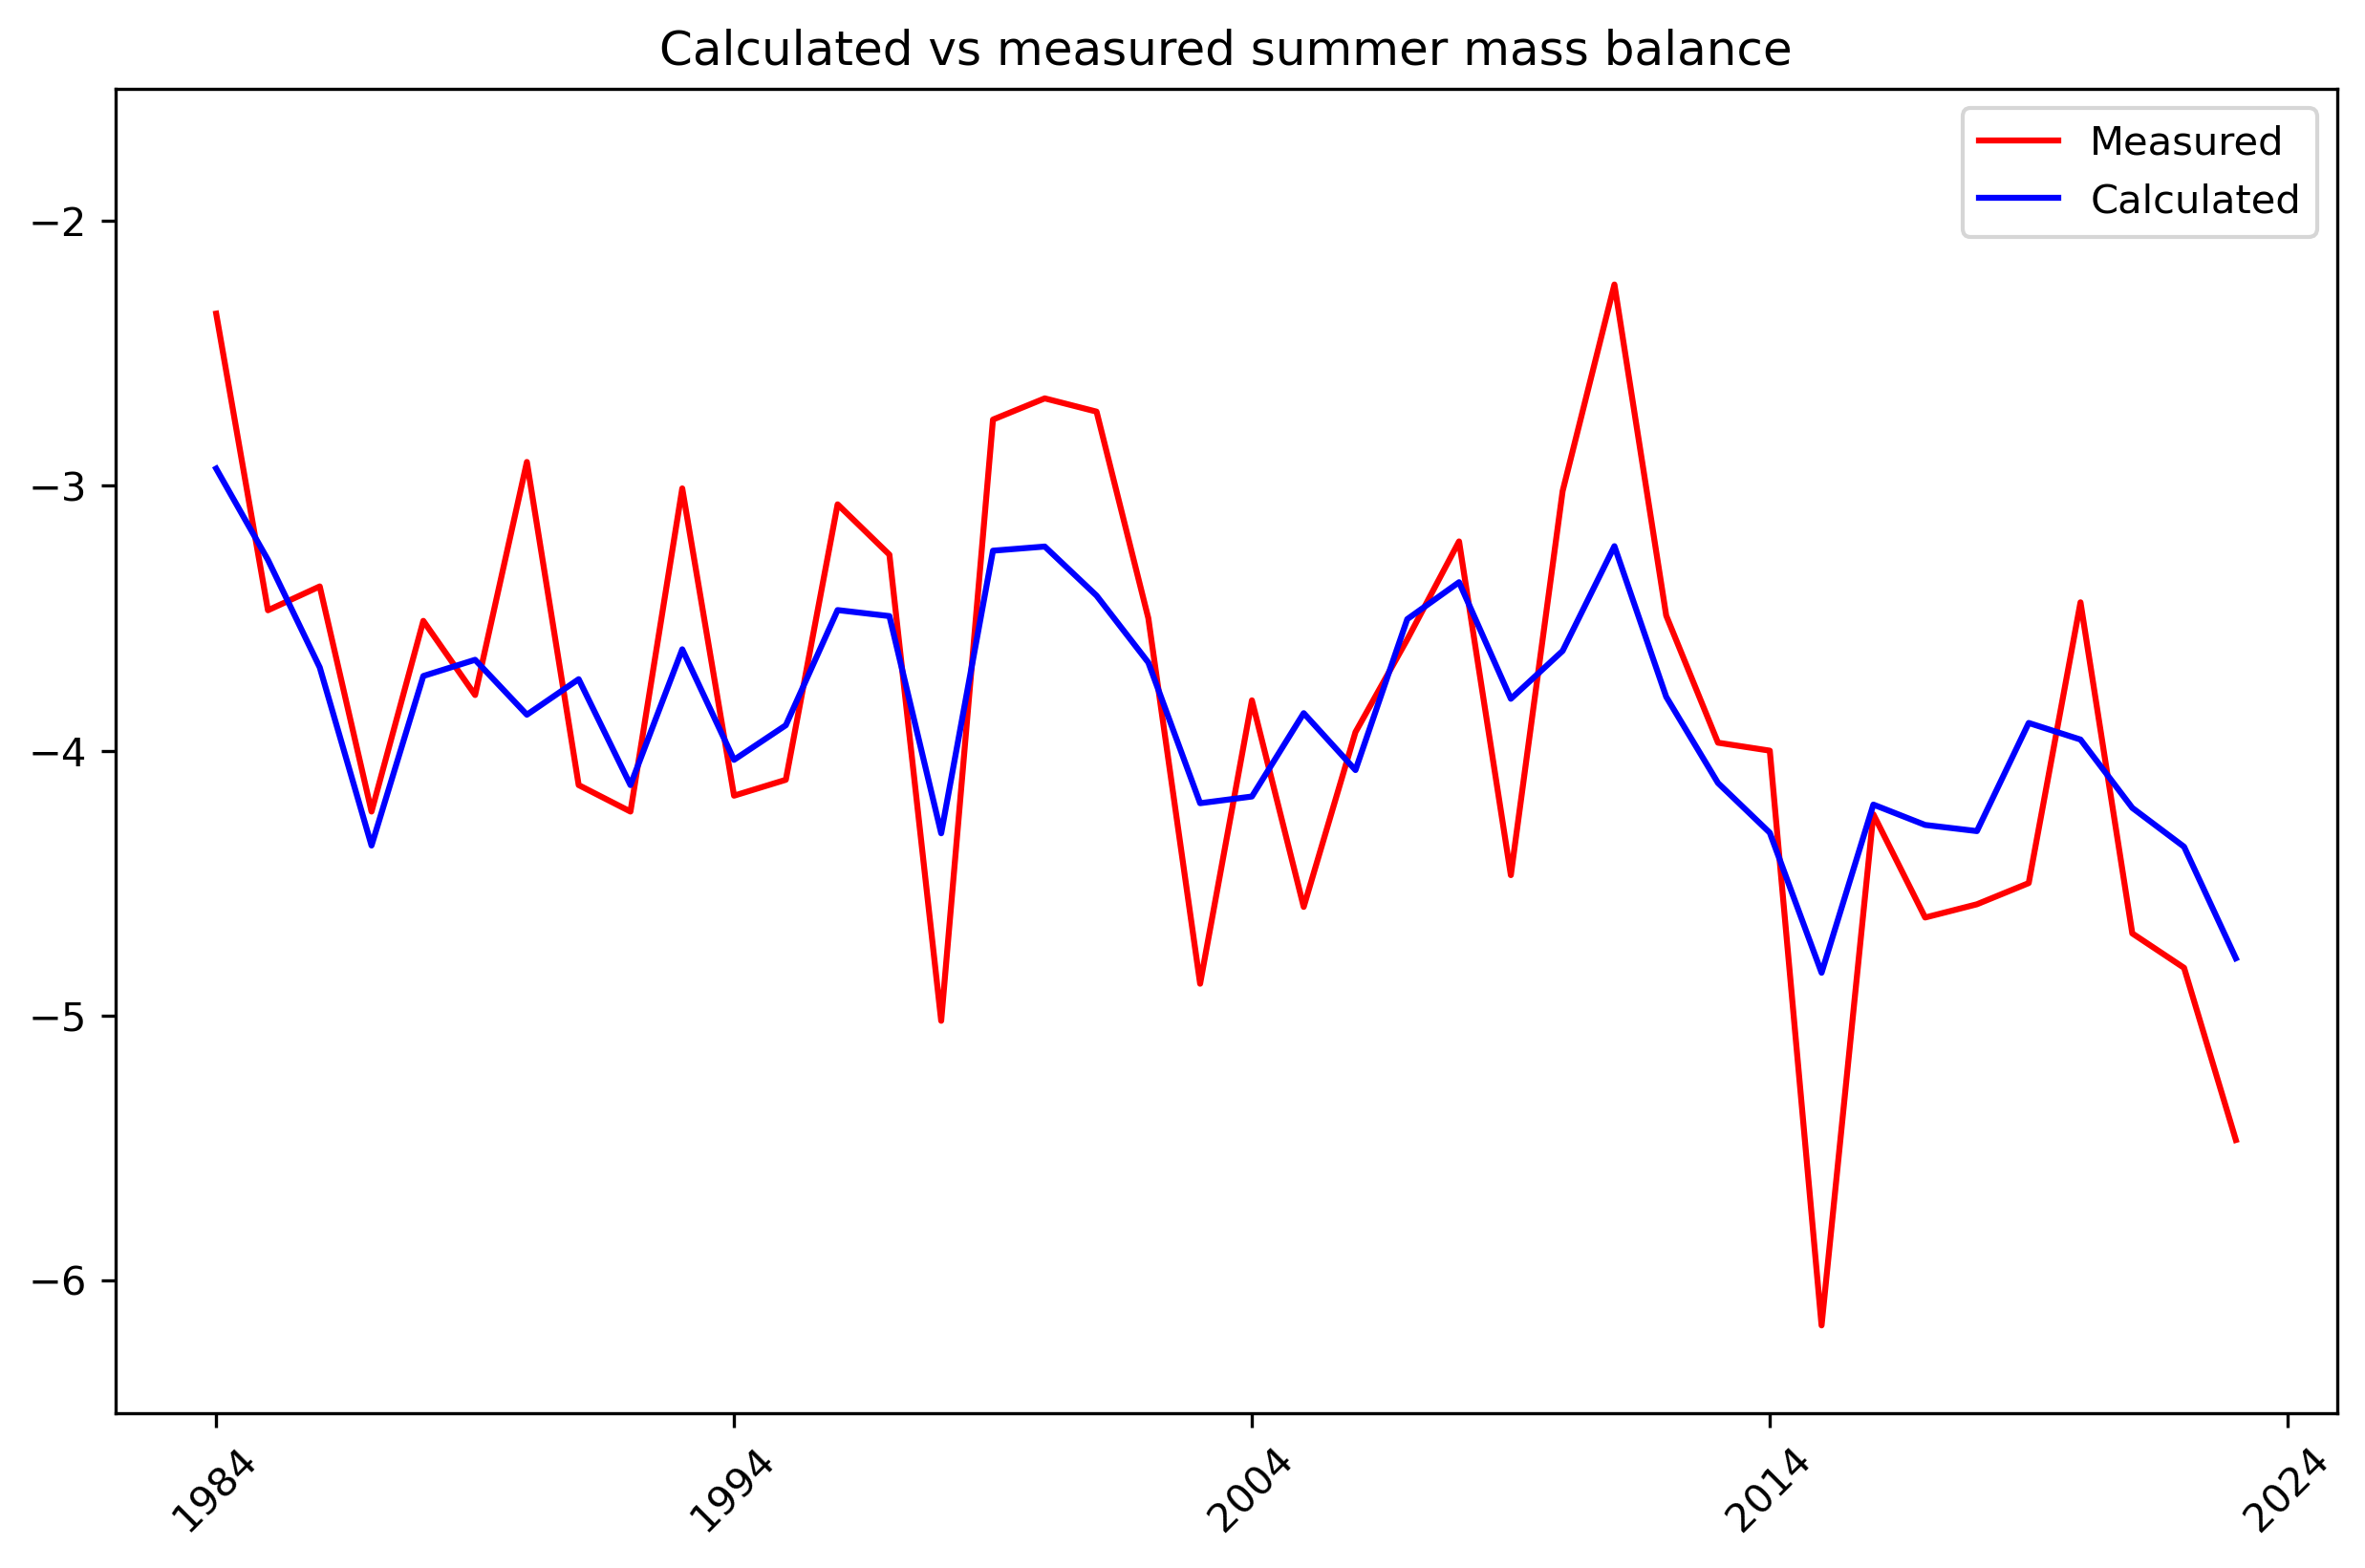
\includegraphics[width=\textwidth]{Plots/summer_mb_compare.png}
        \label{fig:summer_mb_compare}
    \end{subfigure}
    \caption{Comparison plots of the modeled vs measured winter and summer mass balance.}
    \label{fig:mb_comparison}
\end{figure}
\FloatBarrier
\subsection{Runoff Model Error}
The largest problem with the runoff model lies with the precipitation model. This model calculates the type of precipitation that falls (rain or 
snow), based on the temperature. It assumes that if the temperature is greater than $0^\circ$ Celsius then the precipitation is rain, and if the 
temperature is less then $0^\circ$ Celsius then then precipitation is snow. While this is a good generalization it is not always true as precipitation 
can fall as snow when the temperature is right above $0^\circ$ Celsius and vice versa. 
Additionally there is some amount of error in the calculated lapse rate which 
can effect the calculated temperature at the glacier. When the actual temperature at the glacier is right around 0, and precipitation is falling, 
the error in the lapse rate can cause the precipitation to fall as the wrong type. 
\paragraph{}
Shown in \hyperref[fig:calc_vs_measured]{Figure~\ref*{fig:calc_vs_measured}}, there is a large difference the modeled and measured runoff in November 1995. This is likely due to the model predicting the large amount of precipitation 
during that month falling as snow because the model temperatures are just below $0^\circ$ Celsius, but in reality it most likely fell as rain. This also 
highlights the types of error that can be caused by using a proxy weather station that is not present at the glacier such as this model used. With 
more accurate temperature data for the glacier, then the model might correctly predict the precipitation falling as rain. 
\paragraph{}
It is also important to note that out of the 298 missing days of temperature and 292 missing days of precipitation 63 days of temperature and 64 
days of precipitation were during the 1992-2007 period where runoff data is available. Most notable of these missing days is the month of September 
1997. This entire month is missing temperature and precipitation data, and this entire month is included in the measured runoff data. Looking at the 
error for the month it has a relative RMSE of 30.51\% which is very close to the overall relative RMSE of 29.26\%. This 
means that the error this month is quite typical for the model. The interpolated temperatures for this month range from $10^\circ$ C to $5^\circ$ 
during the month, so the glacier is melting and no glacier accumulation is missed. As shown in Figure 7, during September glacier melt is 
contributing the majority of the runoff to the basin, so having zero precipitation in the model for September 1997 would not cause as much error as 
if there was no precipitation for December or January when lack of snowfall could affect the runoff in the following summer.
\begin{figure}[h!]
    \centering
    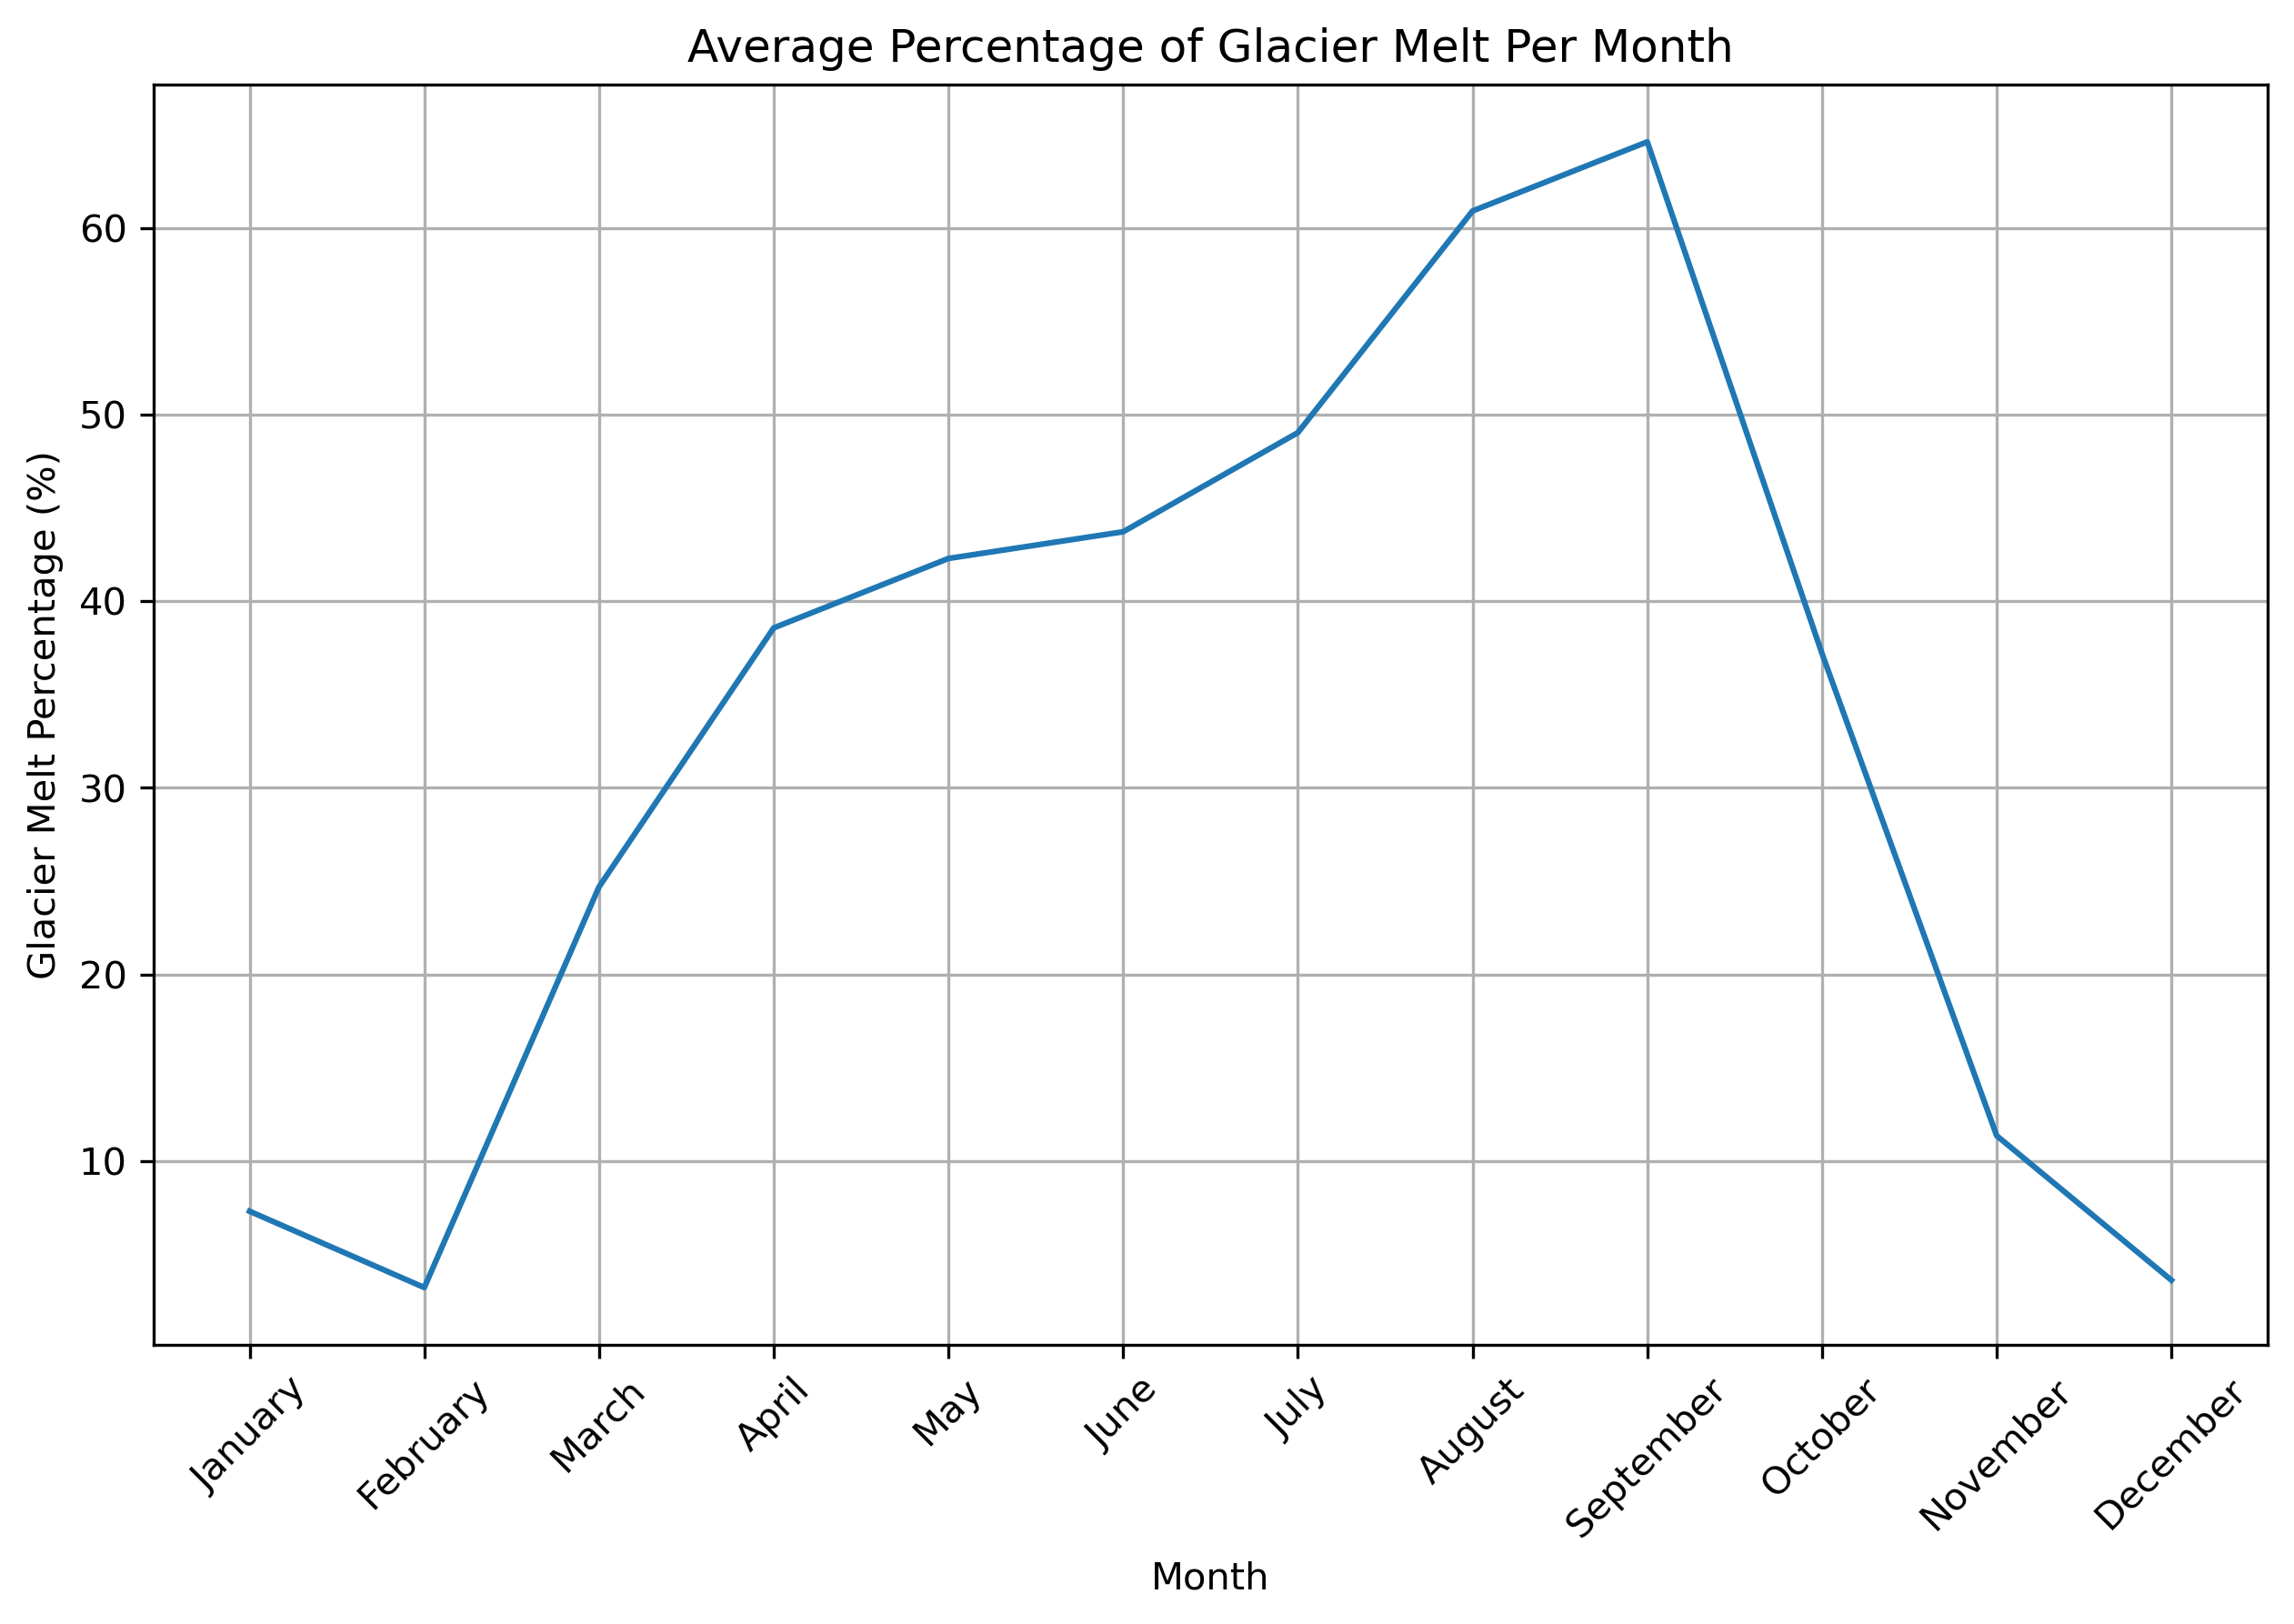
\includegraphics[width=\textwidth]{Plots/percent_glac_melt_month.png}
    \caption{Average percentage from 1984-2024 that the glacier (ice and snow melt) contributes to the monthly runoff}
    \label{fig:percent_glacier_runoff}
\end{figure}
\FloatBarrier
These two examples illustrate that missing precipitation data may be much more detrimental to model accuracy than missing temperature data, 
due to temperature data being much easier to interpolate than precipitation data.
\subsection{Interpretations of Model Results}
Even though the glacier is contributing slightly less than half of the total basin runoff on average (47.56\%), it contributes much more during the summer 
months as show in Figure 7. Due to the setup of the mass balance model there is no way to easily distinguish how much of the glacier melt is made 
up of glacial ice melting and snow melting off the surface of the glacier. So while Figure 7 shows the average monthly percent of runoff due to glacier 
melt, part of that is snow melting off the glacier surface. 
\paragraph{}
As the glacier retreats it will contribute less and less water to the basin runoff resulting in a decrease in total runoff. With a smaller glacier 
surface area the peak snow melt will shift earlier in the summer as the snow melts off faster due the more snow accumulating on rocky surfaces, and not glacier 
ice which keeps the snow cool throughout the summer. As shown in Figure 7, the peak of the glacier runoff occurs in September, which coincides 
with some of the lowest average monthly precipitation amounts as shown in Figure 8.

\begin{figure}[h!]
    \centering
    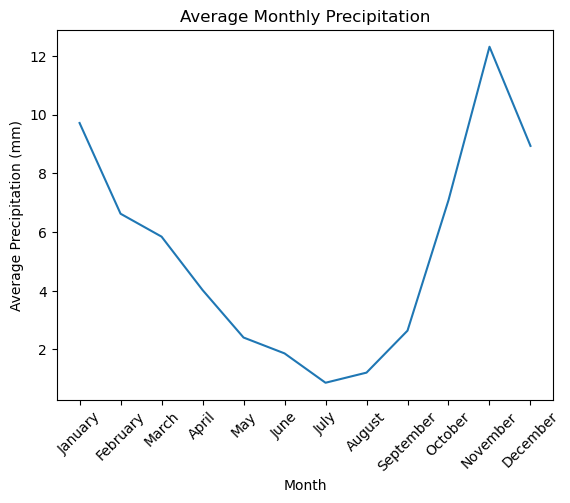
\includegraphics[width=\textwidth]{Plots/monthly_precip.png}
    \caption{Average amount of precipitation per month from 1984-2024 at the Diablo Dam weather station. The average temperature from October-April is below $0^\circ$ C at the glacier, so the precipitation during those months is mostly snow}
    \label{fig:monthly_precip}
\end{figure}    
\FloatBarrier
\textbf{Add paragraph about how the model does on longer timescales. I think I had a paragraph about this before, look for it on github}
\subsection{Overall Model Performance}\textbf{Add paragraph about sia model performing well}
\subsection{Implications of Research}
\subsubsection{Importance of Simplified Ice Dynamics in Numerical Glacier Modeling}
These results show that complicated and computationally intensive mass balance and ice dynamics are not required to accurately model the 
runoff from small mountain glaciers. This means that we can use much simpler and less computationally intensive models such as the ones used 
in this paper to model the runoff from mountain glaciers much quicker than more complicated models. The modeling techniques used in this paper could 
easily be scaled to a much larger region if mass balance is available to tune the input parameters. Also the relative simplicity of the model used in 
this paper means that it is much easier to modify to add new features and customize to a specific region or glacier.
\paragraph{}
This point is further proved by the runoff error of the SIA-Mass Balance model not changing significantly (less than 0.01 for the KGE and NSE, and less than 
0.1\% for the relative RMSE) when 
the ice flux is set to 0. This means that the ice dynamics of the glacier are not a significant factor contributing to the accuracy of the glacier runoff. One reason 
for this is the South Cascade Glacier is in an active state of retreat which can be seen in the model and the 
glacier outline in Figure 1. Since it is retreating, the model does not need the ice dynamics in order to move more glacier ice into the ablation zone 
where it can melt, since much of the glacier is already in this zone.
\subsubsection{Applications}
The work of this paper shows that complex ice dynamics and precipitation models are not always required to accurately model the runoff from small mountain glaciers. This 
can have applications in everything from regional glacier modeling to water resource management as glaciers are a significant source of water 
for many communities around the world. 
\section{Future Work}
As addressed in earlier sections, this model has limited performance on shorter timescales (less than a year). A large portion of these limitations 
are probably due to the precipitation model. The easiest way to improve this would be to have more accurate temperature and precipitation data at the glacier, but 
there are some ways the model could be improved as well. For instance having a dry and wet temperature lapse rate for each month could improve the accuracy of the modeled 
temperature at the glacier. Also the missing precipitation data could be filled in using a supplementary data source or an average monthly precipitation amount.
Additionally increasing the resolution of the model could help improve accuracy but would also increase the runtime.
\paragraph{}
The next step for this project would be to run the model for a glacier near the South Cascade Glacier with a similar climate to see how region specific the input 
parameters are. Due to the input parameters being tuned for the mass balance of the glacier which largely depends on the local climate, it 
is plausible that they could work well for a glacier with a similar climate.
\paragraph{}
Another idea to explore is to run the model with modeled climate data in order to run it into the future to see how this glacier 
will evolve and how the basin runoff will evolve. As shown in (Fountain \& Tangborn, 1985), the peak runoff of a glacierized basin is a function of 
how much of the basin is glacierized. It would be interesting to see how the peak runoff of this basin shifts as the glacier retreats when the model 
is run into the future.
\section{Conclusion}
To answer the thesis question of this paper--yes--a simple SIA - Mass Balance model can be used to model the runoff from small mountain glaciers, but 
it works best on longer timescales.
The SIA-Mass Balance model is able to model the runoff from the South Cascade Glacier with a RMSE, NSE and KGE of 29.26\%, 0.81 and 0.88 respectively, 
for 16 months from 1992-2007, while OGGM errors of 45.96\%, 0.53 and 0.72 for the same time period. 
\textbf{fix these next two sentences}
This show that complex models are not always 
the best way to model the runoff from small mountain glaciers. A simpler model with parameters tuned to the local climate of the glacier can 
perform just as well, if not better than a more complex model. 
\paragraph{}
From looking at the model error on various time scales, one can see that on longer time scales the SIA-Mass Balance model does quite well. More 
advanced models may be able to model the runoff on shorter timescales with more advanced methods and higher model resolution, but simple models 
like the one used in this study can work well on longer (yearly to decade) timescales.
\textbf{add better concluding paragraph}

\section*{Appendix}\
\textbf{Add the rest of the model params}
\begin{table}[h!]
    \centering
    \begin{tabular}{|c|c|c|c|c|c|}
        \hline
        Parameter & $M_s$ &$M_i$ & ${Accum}_l$ & ${Accum}_u$ & Avalanche percentage \\
        \hline
        Value & -0.00316 & -0.00314 & 0.94 & 1.44 & 32\%  \\
        \hline
    \end{tabular}
    \caption{Model Input Parameters}
    \label{tab:model_input_parameters}
\end{table}

\section*{Acknowledgements}
Thanks to the foresight of the USGS in creating the Benchmark Glacier Program in the 1950s to study and document the South Cascade glacier, 
and eventually four more glaciers, there is an abundant amount of information on these glaciers. Due to this program this study was able to 
easily access and use temperature, precipitation, mass balance and DEM data from the USGS. Also as part of this Benchmark Glacier program a 
stream gauge was installed just below the glacier to track the runoff from the basin, the data from which was essential to this project.

Thank you to Robert Jacobel for providing the bed topography data for the South Cascade Glacier, which was essential to this project.

\begin{thebibliography}{}

    % A
    \bibitem{ref1}
    Amaral, T., Bartholomaus, T. C., \& Enderlin, E. M. (2020). Evaluation of iceberg calving models against observations from Greenland outlet glaciers. *Journal of Geophysical Research: Earth Surface, 125*(6), e2019JF005444. https://doi.org/10.1029/2019JF005444

    % B
    \bibitem{ref2}
    Baker, E. H., McNeil, C. J., Sass, L. C., Peitzsch, E. H., Florentine, C. E., Whorton, E. N., O’Neel, S. R., Fagre, D. B., Clark, A. M., \& Miller, Z. S. (2018). USGS Benchmark Glacier Mass Balance and project data [Data release]. https://doi.org/10.5066/F7BG2N8R

    \bibitem{ref3}
    Barnett, T. P., Adam, J. C., \& Lettenmaier, D. P. (2005). Potential impacts of a warming climate on water availability in snow-dominated regions. *Nature, 438*(7066), 303–309. https://doi.org/10.1038/nature04141

    \bibitem{ref4}
    Bidlake, W. R., Josberger, E. G., \& Savoca, M. E. (2004). Water, ice, and meteorological measurements at South Cascade Glacier, Washington, balance year 2002 (Scientific Investigations Report 2004-5089). U.S. Geological Survey. https://doi.org/10.3133/sir20045089
    
    \bibitem{ref5}
    Bidlake, W. R., Josberger, E. G., \& Savoca, M. E. (2005). Water, ice, and meteorological measurements at South Cascade Glacier, Washington, balance year 2003 (Scientific Investigations Report 2005-5210). U.S. Geological Survey. https://doi.org/10.3133/sir20055210

    \bibitem{ref6}
    Bidlake, W. R., Josberger, E. G., \& Savoca, M. E. (2007). Water, ice, and meteorological measurements at South Cascade Glacier, Washington, balance years 2004 and 2005 (Scientific Investigations Report 2007-5055). U.S. Geological Survey. https://doi.org/10.3133/sir20075055

    \bibitem{ref7}
    Bidlake, W. R., Josberger, E. G., \& Savoca, M. E. (2010). Modeled and measured glacier change and related glaciological, hydrological, and meteorological conditions at South Cascade Glacier, Washington, balance and water years 2006 and 2007 (Scientific Investigations Report 2010–5143). U.S. Geological Survey. https://doi.org/10.3133/sir20105143

    % E
    \bibitem{ref8}
    Eis, A., Bahr, D. B., O’Neel, S., \& Elsberg, D. H. (2021). Reconstruction of past glacier changes with an ice-flow glacier model: Proof of concept and validation. *Frontiers in Earth Science, 9*, 595755. https://doi.org/10.3389/feart.2021.595755

    \bibitem{ref9}
    Environmental Systems Research Institute. (2011). *ArcGIS Desktop: Release 10* (Geostatistical Analyst extension—Kriging interpolation). Redlands, CA: ESRI.

    % F
    \bibitem{ref10}
    Farinotti, D., Huss, M., Bauder, A., Funk, M., Truffer, M., \& Gillet-Chaulet, F. (2020). Results from the Ice Thickness Models Intercomparison eXperiment Phase 2 (ITMIX2). *Frontiers in Earth Science, 8*, 571923. https://doi.org/10.3389/feart.2020.571923

    \bibitem{ref11}
    Fountain, A. G., \& Jacobel, R. W. (1997). Advances in ice radar studies of a temperate alpine glacier, South Cascade Glacier, Washington, USA. *Annals of Glaciology, 24*, 303–308. https://doi.org/10.3189/S0260305500014292

    \bibitem{ref12}
    Fountain, A. G., \& Tangborn, W. V. (1985). The effect of glaciers on streamflow variations. *Water Resources Research, 21*(4), 579–586. https://doi.org/10.1029/WR021i004p00579

    % G
    \bibitem{ref13}
    GlaThiDa Consortium. (2020). *Glacier Thickness Database 3.1.0* [Data set]. World Glacier Monitoring Service. https://doi.org/10.5904/wgms-glathida-2020-10

    \bibitem{ref14}
    GLIMS Consortium. (2005). *GLIMS Glacier Database (Version 1)* [Data set]. National Snow and Ice Data Center. https://doi.org/10.7265/N5V98602

    % H
    \bibitem{ref15}
    Harris, C. R., Millman, K. J., van der Walt, S. J., et al. (2020). Array programming with NumPy. *Nature, 585*(7825), 357–362. https://doi.org/10.1038/s41586-020-2649-2

    % I
    \bibitem{ref16}
    Iken, A. (1981). The effect of the subglacial water pressure on the sliding velocity of a glacier in an idealized numerical model. *Journal of Glaciology, 27*(97), 407–421. https://doi.org/10.3189/S0022143000011448

    % K
    \bibitem{ref17}
    Kessler, M. A., Anderson, R. S., \& Stock, G. M. (2006). Modeling topographic and climatic control of east–west asymmetry in Sierra Nevada glacier length during the Last Glacial Maximum. *Journal of Geophysical Research, 111*, F02002. https://doi.org/10.1029/2005JF000365

    \bibitem{ref18}
    Krimmel, R. M. (1993). Mass balance, meteorological, and runoff measurements at South Cascade Glacier, Washington, 1992 balance year (Open-File Report 93-640). U.S. Geological Survey. https://doi.org/10.3133/ofr93640

    \bibitem{ref19}
    Krimmel, R. M. (1994). Runoff, precipitation, mass balance, and ice velocity measurements at South Cascade Glacier, Washington, 1993 balance year (Water-Resources Investigations Report 94-4139). U.S. Geological Survey.

    \bibitem{ref20}
    Krimmel, R. M. (1995). Water, ice, and meteorological measurements at South Cascade Glacier, Washington, 1994 balance year (Water-Resources Investigations Report 95-4162). U.S. Geological Survey.

    \bibitem{ref21}
    Krimmel, R. M. (1996). Water, ice, and meteorological measurements at South Cascade Glacier, Washington, 1995 balance year (Water-Resources Investigations Report 96-4174). U.S. Geological Survey.

    \bibitem{ref22}
    Krimmel, R. M. (1997). Water, ice, and meteorological measurements at South Cascade Glacier, Washington, 1996 balance year (Water-Resources Investigations Report 97-4143). U.S. Geological Survey.

    \bibitem{ref23}
    Krimmel, R. M. (1998). Water, ice, and meteorological measurements at South Cascade Glacier, Washington, 1997 balance year (Water-Resources Investigations Report 98-4090). U.S. Geological Survey.

    \bibitem{ref24}
    Krimmel, R. M. (1999). Water, ice, meteorological and speed measurements at South Cascade Glacier, Washington, 1998 balance year (Water-Resources Investigations Report 99-4049). U.S. Geological Survey.

    \bibitem{ref25}
    Krimmel, R. M. (2001). Water, ice, meteorological, and speed measurements at South Cascade Glacier, Washington, 1999 balance year (Water-Resources Investigations Report 00-4265). U.S. Geological Survey.

    \bibitem{ref26}
    Krimmel, R. M. (2002). Water, ice, and meteorological measurements at South Cascade Glacier, Washington, 2000–01 balance years (Water-Resources Investigations Report 02-4165). U.S. Geological Survey.

    % L
    \bibitem{ref27}
    Lange, S., Menz, C., Gleixner, S., Cucchi, M., Weedon, G. P., Amici, A., Bellouin, N., Müller-Schmied, H., Hersbach, H., \& Buontempo, C. (2021). WFDE5 over land merged with ERA5 over the ocean (W5E5 v2.0) [Data set]. ISIMIP. https://doi.org/10.48364/ISIMIP.342217

    \bibitem{ref28}
    Le Meur, E., Gagliardini, O., Zwinger, T., \& Ruokolainen, J. (2004). Glacier flow modelling: A comparison of the shallow ice approximation and the full-Stokes solution. *Comptes Rendus Physique, 5*(7), 709–722. https://doi.org/10.1016/j.crhy.2004.10.001

    \bibitem{ref29}
    Le Meur, E., \& Vincent, C. (2003). A two-dimensional shallow ice-flow model of Glacier de Saint-Sorlin, France. *Journal of Glaciology, 49*(167), 527–538. https://doi.org/10.3189/172756503781830421

    % M
    \bibitem{ref30}
    Maussion, F., Butenko, A., Champollion, N., Dusch, M., Eis, J., Fourteau, K., Gregor, P., Jarosch, A. H., Landmann, J., Oesterle, F., Recinos, B., Rothenpieler, T., Vlug, A., Wild, C. T., \& Marzeion, B. (2019). The Open Global Glacier Model (OGGM) v1.1. *Geoscientific Model Development, 12*(3), 909–931. https://doi.org/10.5194/gmd-12-909-2019

    \bibitem{ref31}
    McNeil, C. J., Florentine, C. E., Bright, V. A. L., Fahey, M. J., McCann, E., Larsen, C. F., Thoms, E. E., Shean, D. E., McKeon, L. A., March, R. S., Keller, W., Whorton, E. N., O’Neel, S., Baker, E. H., Sass, L. C., \& Bollen, K. E. (2019). Geodetic data for USGS benchmark glaciers: Orthophotos, digital elevation models, glacier boundaries and surveyed positions (ver. 3.0, August 2022) [Data release]. U.S. Geological Survey. https://doi.org/10.5066/P9R8BP3K

    % N
    \bibitem{ref32}
    Naz, B. S., Frans, C. D., Clarke, G. K. C., Burns, P., \& Lettenmaier, D. P. (2014). Modeling the effect of glacier recession on streamflow response using a coupled glacio-hydrological model. *Hydrology and Earth System Sciences, 18*, 787–802. https://doi.org/10.5194/hess-18-787-2014

    % P
    \bibitem{ref33}
    PRISM Group, Oregon State University. (2014). PRISM climate data. https://prism.oregonstate.edu

    % R
    \bibitem{ref34}
    Rasmussen, L. A. (2009). South Cascade Glacier mass balance, 1935–2006. *Annals of Glaciology, 50*(50), 215–220. https://doi.org/10.3189/172756409787769755

    % U
    \bibitem{ref35}
    U.S. Geological Survey Benchmark Glacier Program. (2020). USGS benchmark glacier project comprehensive data collection [Data release]. https://doi.org/10.5066/P9AGXQSR

    % V
    \bibitem{ref36}
    Virtanen, P., Gommers, R., Oliphant, T. E., et al. (2020). SciPy 1.0: Fundamental algorithms for scientific computing in Python. *Nature Methods, 17*(3), 261–272. https://doi.org/10.1038/s41592-019-0686-2

\end{thebibliography}
  

\end{document}
